\chapter{Grafteori}
Følgende kapitel er skrevet med afsæt i \citep{dmat}.

Grafer er diskrete strukturer bestående af et antal knuder, også betegnet punkter, samt et antal kanter, der forbinder disse knuder. Knuderne illustreres ofte som prikker, mens kanterne repræsenteres af streger eller pile, der forbinder disse prikker. Graferne varierer alt efter deres type og funktion. De mange forskellige egenskaber betyder, at problemer i næsten enhver tænkelig disciplin kan løses ved hjælp af grafmodeller. Vi vil eksempelvis i dette projekt benytte grafteori og princippet om den længste vej til at optimere et gaslager.

\section{Graftyper}
En graf er, som tidligere nævnt, en struktur med punkter og kanter. Den er givet ved definitionen:
\begin{definition}
[Graf] 
En graf $G=(V,E)$ består af $V$, en punktmængde, hvor $V\neq0$, og en kantmængde; $E \subseteq \{\{u;v\}|u,v \in V\}$.
\end{definition}
Det fremgår af definitionen, at en graf ikke kan have 0 punkter, men en lignende afgrænsning i den anden ende eksisterer ikke. Der kan altså godt være uendeligt mange knuder og kanter. I så fald kaldes det en uendelig graf. Ellers kaldes det en endelig graf, og det er denne type, som vi beskæftiger os med i projektet.
Ydermere, ses det i definitionen, at hver kant forbinder én eller to punkter. For en simpel graf gælder det, at ingen kanter forbinder et punkt med sig selv. Der må altså ikke være løkker. Derudover forbindes to punkter med max én kant.
\begin{figure}[H]
\centering
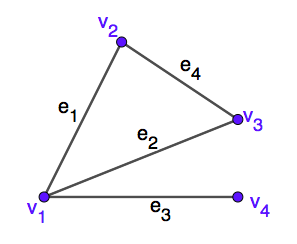
\includegraphics[scale=0.5]{fig/img/simpel_graf.png}
\caption{En simpel graf}
\label{fig:simpel}
\end{figure}
I kontrast til den simple graf finder vi multi-grafen. For denne type graf skal der være flere kanter, der forbinder det samme sæt punkter. Der må stadig ikke optræde løkker.
\begin{figure}[H]
\centering
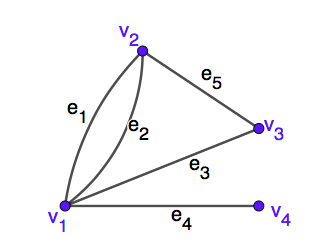
\includegraphics[scale=0.5]{fig/img/multigraf.png} 
\caption{En multigraf}
\label{fig:multi}
\end{figure}
I eksemplet ovenover ses det, at to kanter forbinder punktsættet ($v_{1},v_{2}$). Hvis en graf, modsat de to allerede nævnte, kan indeholde både løkker og flere kanter, der forbinder de samme punkter, kaldes det en pseudo-graf. Vi ser i eksemplet herunder, at der er to kanter, der forbinder $v_{1}$ og $v_{2}$, og der er en løkke ved $v_{4}$.
\begin{figure}[H]
\centering
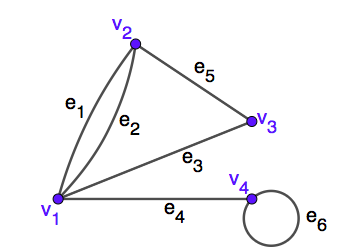
\includegraphics[scale=0.5]{fig/img/pseudograf.png}
\caption{En pseudograf med et loop}
\label{fig:pseudo}
\end{figure}
En anden grafopdeling man kan 
\subsection{Orienterede grafer og ikke-orienterede grafer}
En anden typisk grafopdeling er opdelingen i orienterede og ikke-orienterede grafer. De grafer vi har kigget på indtil videre er ikke-orienterede grafer. For en orienteret graf gælder det, at dets kanter har en retning. Dette er ofte illustreret med pile. Den har dermed et startpunkt og et endepunkt. Disse grafer er defineret ved:
\begin{definition}
[Orienteret graf] 
En orienteret graf $(V,E)$ består af $V$, et sæt punkter(knuder), hvor $V\neq0$, og et sæt orienterede kanter, $E$. Hver orienterede kant forbinder et sæt punkter $(u,v)$, hvor $u$ er tilstødende til $v$, og $v$ er tilstødende fra $u$. Punktet $u$ kaldes begyndelsespunktet, og punktet $v$ kaldes endepunktet.
\end{definition}
\begin{figure}[H]
\centering
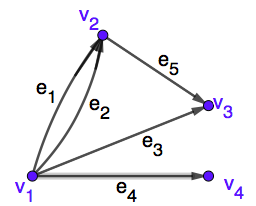
\includegraphics[scale=0.5]{fig/img/orienteret_graf.png}
\caption{En orienteret graf}
\label{fig:orienteret}
\end{figure}
Der kan foruden disse to også være tale om mixede grafer, som er grafer med både orienterede og ikke-orienterede kanter. Orienterede grafer kan ligesom ikke-orienterede grafer indeholde loops og flere kanter der forbinder det samme punktsæt. Den må også indeholde to modsatrettede kanter mellem det samme punktpar. Dvs. en kant må gerne gå fra $v$ til $u$, selvom en anden kant går fra $u$ til $v$. Hvis en orienteret graf hverken indeholder loops eller flere kanter, der forbinder det samme punktpar, kaldes den en orienteret simpel graf. Hvis der derimod optræder flere kanter mellem et eller flere punktpar, kaldes det en multigraf.Vi kan se egenskaberne for de forskellige grafer herunder:

\begin{tabular}{ |p{4cm}||p{3cm}|p{3cm}|p{2cm}|  }
 \hline
 \multicolumn{4}{|c|}{Grafer} \\
 \hline
 Type & Kanter & Flere Kanter pr punktpar tilladt? & Løkker tilladt\\
 \hline
 Simpel graf   & Ikke-orienteret    & Nej &   Nej\\
 Multigraf &   Ikke-orienteret & Ja   & Nej\\
 Pseudograf & Ikke-orienteret & Ja &  Ja\\
 Simpel orienteret graf    & Orienteret & Nej &  Nej\\
 Orienteret multigraf &  Orienteret  & Ja & Ja\\
 Mixet graf & Ikke-orienteret og orienteret  & Ja   & Ja\\
 \hline
\end{tabular}

Fordi kanterne i grafer med orienterede kanter er ordnede par kan definitionen af punktets grader være antallet af kanter, der har dette punkt som begyndelsespunkt, eller antallet af kanter, der har dette punkt som endepunkt:
\begin{definition}
[Graden af en orienteret graf] 
I en graf med orienterede kanter er ind-graden, betegnet ved $deg^{-}(v)$, antallet af kanter med v som deres endepunkt. Ud-graden, betegnet ved $deg^{+}(v)$, er antallet af kanter med v som deres startpunkt.
\end{definition}
Vi vil i projektet beskæftige os med orienterede grafer, da det er denne type vi bruger til optimeringen af gaslageret. I vores tilfælde vil vi tildele vores orienterede kanter vægt, hvilket beskrives senere i projektet.

\input{incl/main/grafer/repræsentation}
\subsection{Nabolister}
En måde at repræsentere en graf på er ved at lave en naboliste. Nabolister er tabeller, der giver en oversigt over hvilke knuder, der er forbundet med andre knuder. Dog vil man ikke kunne se, hvis der er parallelle kanter. En naboliste er bygget op således, at knuden, man vil beskrive, er i venstre side af tabellen, og naboknuderne er skrevet i højre side. \\

\begin{figure}[h]
  \centering
  \begin{tikzpicture}
    \node[point] at (1,2) (A) [label=above:\(A\)] {};
    \node[point] at (3,2) (B) [label=above:\(B\)] {};
    \node[point] at (4,1) (C) [label=right:\(C\)] {};
    \node[point] at (2,0) (D) [label=below:\(D\)] {};
    \node[point] at (3,0) (E) [label=below:\(E\)] {};
    \node[point] at (1,1) (F) [label=left:\(F\)] {};
    \node[point] at (0,2) (G) [label=below:\(G\)] {};

    \footnotesize
    \draw (A) -- (G);
    \path (F) edge [bend left] (B);
    \draw (A) -- (F);
    \path (F) edge [bend right] (B);
    \draw (B) -- (D);
    \draw (B) -- (E);
    \draw (B) -- (C);
    \draw (C) -- (E);
    \draw (C) to [out=315,in=45,looseness=50] (C);
    \draw (E) -- (D);
    \draw (D) -- (F);
    \draw (F) -- (G);
  \end{tikzpicture}
  \caption{Ikke-orienteret pseudograf.}
  \label{fig:ikke-orienteret-pseudo}
\end{figure}

\begin{center}
	\begin{tabular}{ |p{4cm}||p{3cm}|}
	 	\hline
 		\multicolumn{2}{|c|}{Naboliste til figur \ref{fig:ikke-orienteret-pseudo}} \\
 		\hline
 		Knuder & Naboknuder\\
 		\hline
 		A & F,G \\
		B & C,D,E,F \\
		C & B,E,C \\
		D & B,E,F \\
		E & B,C,D \\
		F & A,B,D,G \\
		G & A,F \\
 	\hline
 	\label{tab:naboliste} 	
	\end{tabular}
	%\caption{Naboliste til figur \ref{fig:ikke-orienteret-pseudo}
\end{center}
Ud fra tabellen ses, at knuden B har naboknuderne C, D, E og F, men man kan ikke se, at der er en ekstra kant mellem B og F. Dog kan man se, at C har en løkke, da den er nabo til sig selv.

\begin{figure}[H]
  \centering
  \begin{tikzpicture}
    \node[point] at (1,2) (A) [label=above:\(A\)] {};
    \node[point] at (3,2) (B) [label=above:\(B\)] {};
    \node[point] at (4,1) (C) [label=right:\(C\)] {};
    \node[point] at (2,0) (D) [label=below:\(D\)] {};
    \node[point] at (3,0) (E) [label=below:\(E\)] {};
    \node[point] at (1,1) (F) [label=left:\(F\)] {};
    \node[point] at (0,2) (G) [label=below:\(G\)] {};

    \footnotesize
    \path [->] (A) edge [bend left] (G);
    \path [->] (A) edge [bend right] (G); 
    \path [->] (F) edge [bend left] (B);
    \draw [<-](A) -- (F);
    \path [<-](F) edge [bend right] (B);
    \draw [->](B) -- (D);
    \draw [<-](B) -- (E);
    \draw [<-](B) -- (C);
    \draw [->](C) -- (E);
    \draw [->](C) to [out=315,in=45,looseness=50] (C);
    \draw [<-](E) -- (D);
    \draw [->](D) -- (F);
    \draw [->](F) -- (G);
  \end{tikzpicture}
  \caption{Orienteret pseudograf.}
  \label{fig:orienteret-pseudo}
\end{figure}

%\begin{center}
%	\begin{tabular}{ |p{4cm}||p{3cm}|}
%	 	\hline
% 		\multicolumn{2}{|c|}{Naboliste til figur \ref{fig:orienteret-pseudo} \\
% 		\hline
% 		Knuder & Naboknuder\\
% 		\hline
% 		A & G \\
%		B & D,F \\
%		C & B,E,C \\
%		D & E,F \\
%		E & B \\
%		F & A,B,G \\
%		G &  \\
% 	\hline
% 	\label{tab:naboliste1}
%	\end{tabular}
%\end{center}

\ref{tab:naboliste1} viser en oversigt over den orienterede grafs (Figur \ref{fig:orienteret-pseudo}) naboknuder. Kigger man på B og F i tabellen, kan man se, at der er parallelle kanter, da kanterne er orienteret i hver deres retning. Kigger man på A og G, kan man ikke se, at der er parallelle kanter mellem A og G, da begge kanter er orienteret fra A til G.
\subsection{Nabomatricer}
En anden mulighed for at repræsentere en graf er ved brug af nabomatricer. Nabomatricer er bedre, når grafen har mange kanter.\\
En nabomatrice kan beskrives som en $N=m X m$ matrice, hvor $m$ er afhængig af knudemængden $V=\{v_0, v_1, \ldots, v_m\}$. Hvis man har en simpel graf, $G=(V,E)$, vil matricen være en nul-1 matrice, da en simpel graf kan kun have en kant mellem to knuder. Når der er en kant mellem to  vilkårlig knuder, $(v_i,v_j)$,  vil den få notationen 1, hvis der derimod ikke er en kant vil får den notation 0. \\

Det kan også skrives som \\

\begin{equation}
\begin{Bmatrix} 
	 \hspace{0.3cm}\textrm{1 hvis} \hspace{0.3cm}\{v_i,v_j\} \hspace{0.2cm} \textrm{har en kant i grafen} \hspace{0.2cm} G \\
	 \textrm{0 ellers} \\
	\end{Bmatrix}
\end{equation}

\begin{figure}[H]
  \centering
  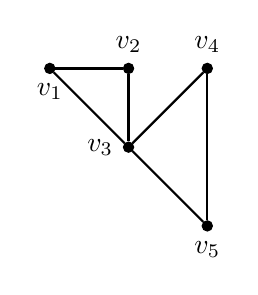
\begin{tikzpicture}
  \tikzset{enclosed/.style={draw, circle, inner sep=0pt, minimum size=.13cm, fill=black}}
  	\node[enclosed] at (0,2) (v1) [label=below:\(v_1\)] {};
    \node[enclosed] at (1,2) (v2) [label=above:\(v_2\)] {};
    \node[enclosed] at (1,1) (v3) [label=left:\(v_3\)] {};
    \node[enclosed] at (2,2) (v4) [label=above:\(v_4\)] {};
    \node[enclosed] at (2,0) (v5) [label=below:\(v_5\)] {};
    
	\path[thick] (v1) edge node {} (v2);
	\path[thick] (v1) edge node {} (v3);
	\path[thick] (v2) edge node {} (v3);
	\path[thick] (v4) edge node {} (v3);
	\path[thick] (v5) edge node {} (v3);   
	\path[thick] (v4) edge node {} (v5); 

  \end{tikzpicture}
  \caption{Ikke-orienteret, simpel graf.}
  \label{fig:stm}
\end{figure}

  \label{fig:simpelgraf}
\end{figure}

Nabo natricen nedenfor bruger rækkefølgen $v_1$,$v_2$,$v_3$,$v_4$,$v_5$
\begin{equation}
	\begin{bmatrix}
		0&1&1&0&0 \\
		1&0&1&0&0 \\
		1&1&0&1&1 \\
		0&0&1&0&1 \\
		0&0&1&1&0 \\
	\end{bmatrix}
\end{equation}

	



\section{Veje}
Vi har indtil videre snakket om kanter, og hvordan de enkeltvis er incidente med knudepar. I dette afsnit vil vi udvide det til at snakke om veje, som er følger af disse kanter, og dermed er de også grafer i sig selv. Hvis der er tale om ikke-orienterede grafer, er veje defineret ved:
\begin{defn}
[Veje i ikke-orienterede grafer] 
Lad $n \in \N _0$  og $G$ være en ikke-orienteret graf. En vej, $P$, af længde $n$, fra $u$ til $v$, i $G$ er en følge af $n$ kanter,  $ P= (e_{1},e_{2},\dotsc,e_{n})$, for hvilken der eksisterer en følge, $u=x_{0}$ og $v=(x_{1},x_{2},\dotsc,x_{n-1}$,$x_{n})$, af knuder sådan at $e_{i}$ har, for $i=1,2,\dotsc,n$, endeknuderne $x_{i-1}$ og $x_{i}$. Når grafen er simpel, betegnes vejen ved grafens knudefølge, $x_{o},x_{1},\dotsc,x_{n}$. Hvis den ikke er simpel, beskrives vejen ved kanterne, $e_{1},e_{2},\dotsc,e_{n}$. 
\end{defn}
Her er en vej simpel, hvis den kun passerer den samme kant én gang. Kigger vi derimod på veje med orienterede grafer, som er det vi beskæftiger os med i problemet, ser definitionen en smule anderledes ud:
\begin{defn}
[Veje i orienterede grafer] 
Lad $n \in \N _0$ og $G$ være en orienteret graf. En vej, $P$, af længde $n$, fra $u = x_0$ til $v = x_n$, i $G$ er en følge af kanter, $e_{1},e_{2},\dotsc,e_{n}$, $ \exists (x_{n-1},x_{n}) $ for $e_{n} \forall e_n$. Hvis alle knudepar, i en given vej, højst har én kant som er incident med parret, betegner vi vejen ved dennes knudefølge $x_{o},x_{1},\dotsc,x_{n}$.
\end{defn}

\begin{figure}[H]
\centering
	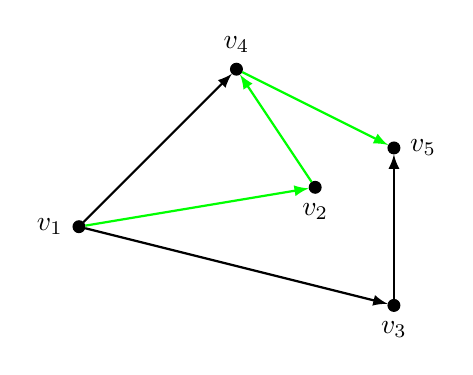
\begin{tikzpicture}

      \tikzset{enclosed/.style={draw, circle, inner sep=0pt, minimum size=.15cm, fill=black}}
%% Vertices
      	\node[enclosed, label={left: $v_1$}] (v1) at (0,2) {};
      	\node[enclosed, label={below: $v_2$}] (v2) at (3,2.5) {};
    		\node[enclosed, label={below: $v_3$}] (v3) at (4,1) {};
  	    \node[enclosed, label={above: $v_4$}] (v4) at (2,4) {};
     	\node[enclosed, label={right: $v_5$}] (v5) at (4,3) {};
%Edges
		\path [->, >=latex, thick, green](v1) edge node[midway, sloped, above] {} (v2);
		\path [->, >=latex, thick](v1) edge node[midway, sloped, above] {} (v3);
		\path [->, >=latex, thick](v1) edge node[midway, above] {} (v4);
		\path [->, >=latex, thick, green](v2) edge node[near end, sloped, below] {} (v4);
		\path [->, >=latex, thick](v3) edge node[midway, below] {} (v5);
		\path [->, >=latex, thick, green](v4) edge node[near end, sloped, above] {} (v5);

	\end{tikzpicture}
	\caption{Eksempel på en orienteret simpel graf og en vej fra $v_{0}$ til $v_{4}$}
	\label{fig.vaegtetopg}
\end{figure}

Antallet af veje mellem to knuder i grafen kan findes ved hjælp af nabomatricer, som vi diskuterede i forrige afsnit.
\begin{thm}
[Antallet af veje mellem to knuder] 
Lad G være en vilkårlig graf med nabomatricen
\textbf{$A$} med grafens knuder i rækkefølgen $v_{1},v_{2},\dotsc,v_{n}$. Antallet af forskellige veje med længde $r$ fra $v_{i}$ til $v_{j}$ vil da være lig den $(i,j)$'te indgang af \textbf{$A^{r}$}.
\end{thm}

\begin{proof}
Bevis: Lad G være en graf med nabomatricen 
\textbf{$A$}, hvor vi antager, at knuderne i $G$ har rækkefølgen $v_{1},v_{2},\cdots,v_{n}$. Antallet af veje fra $v_{i}$ til $v_{j}$ af længde 1 er da den $(i,j)$'te indgang til 
\textbf{$A$}. Dette skyldes, at det blot er antallet af kanter fra $v_{i}$ til $v_{j}$.
Vi antager, at den $(i,j)$'te indgang til 
\textbf{${A^r}$} er antallet af forskellige veje, som går fra $v_{i}$ til $v_{j}$ og som har længden $r$. Dette er hypotesen, vi ønsker at bekræfte.
Vi ser på nabomatricen \textbf{$A^{r+1}$}. 
\textbf{$A^{r+1}$} er det samme som 
\textbf{$A^{r}$}$\dotsc$\textbf{$A$}, og derfor er den $(i,j)$'te indgang af \textbf{$A^{r+1}$} lig med $b_{i1}a_{1j} + b_{i2}a_{2j} +\dotsc+ b_{in}a_{nj}$. Her er $b_{ik}$  den $(i,k)$'te indgang til 
\textbf{$A^{r}$}, som ifølge vores hypotese er antallet af veje fra $v_{i}$ til $v_{k}$ med længde $r$.
En vej af længde $r + 1$ fra $v_{i}$ til $v_{k}$ er lavet ud fra en vej med længden $r$ fra begyndelsesknuden $v_{i}$ og hen til en mellemliggende knude $v_{k}$ samt den kant, der går fra $v_{k}$ til $v_{j}$. Vi ved fra kombinatorik, at antallet af muligheder er lig produktet af mulighederne ved første udfald og mulighederne ved andet udfald. Vi betegner antallet af veje med længden $r$ fra $v_{i}$ til $v_{k}$ med $b_{ik}$ og antallet af kanter fra $v_{k}$ til $v_{j}$ med $a_{kj}$ Finder vi produktet af dette for alle mellemliggende knuder, $v_{k}$, fås det ønskede resultat.
\end{proof}

\begin{exmp}
Vi starter med at kigge på en graf og den tilhørende nabomatrice:
\begin{figure}[H]
\centering
	\begin{tikzpicture}

      \tikzset{enclosed/.style={draw, circle, inner sep=0pt, minimum size=.15cm, fill=black}}
%% Vertices
      	\node[enclosed, label={left: $v_1$}] (v1) at (1,2) {};
      	\node[enclosed, label={above: $v_2$}] (v2) at (3,4) {};
    	\node[enclosed, label={below: $v_3$}] (v3) at (1,0) {};
  	    \node[enclosed, label={right: $v_4$}] (v4) at (5,2) {};
     	\node[enclosed, label={below: $v_5$}] (v5) at (5,0) {};
%Edges
		\path (v1) edge node[midway, sloped, above] {} (v2);
		\path (v1) edge node[midway, sloped, above] {} (v3);
		\path (v1) edge node[midway, above] {} (v4);
		\path (v2) edge node[near end, sloped, below] {} (v4);
		\path (v3) edge node[midway, below] {} (v5);
		\path (v4) edge node[near end, sloped, above] {} (v5);

	\end{tikzpicture}
	\caption{Eksempel på en ikke-orienteret simpel graf}
	\label{fig.vaegtetopg}
\end{figure}

\begin{equation}
A=\begin{bmatrix}
    0&1&1&1&0\\
    1&0&0&1&0\\
    1&0&0&0&1\\
    1&1&0&0&1\\
    0&0&1&1&0\\
\end{bmatrix}
\end{equation}


Vi ønsker at finde ud af hvor mange veje med en længde på 4, der går fra $v_1$ til $v_5$. Det ses i nabomatricen, at $v_1$ har 3 naboer, nemlig $v_2$, $v_3$ og $v_4$. Fortsætter vi, kan vi se, at $v_2$ har $v_1$ og $v_4$ som naboer, $v_3$ har $v_1$ og $v_5$, og $v_4$ har $v_1$, $v_2$ og $v_5$ som naboer. Fortsætter vi, så vi finder alle tænkelige veje med længder på 3, får vi, at der er 18 forskellige veje, der alle starter i $v_1$ og har en længde på 3. Vi skal nu finde de veje, der ved at tilføje en kant, ender i $v_5$. Vi kan se, at $v_5$ har $v_3$ og $v_4$ som naboer. Vi finder derfor de veje, der starter i $v_1$ og slutter i $v_3$, med længden 3, og derefter dem, der slutter i $v_4$, med længden 3. På denne måde udnytter vi, hvad vi skrev i beviset, nemlig at
\textbf{$A^{r+1}$} er lig med $b_{i1}a_{1j} + b_{i2}a_{2j} +\cdots+ b_{in}a_{nj}$
Her er $b_{ik}$ antallet af veje fra $v_{i}$ til ${v_k}$. I vores eksempel er $v_{i}=v_{1}$, ${v_{k1}}=v_{3}$, ${v_{k2}}=v_{4}$, $v_{j}=v_{5}$ og \textbf{$A^{r+1}$}=\textbf{$A^{3+1}$}. 
 
\begin{figure}[H]
\centering
	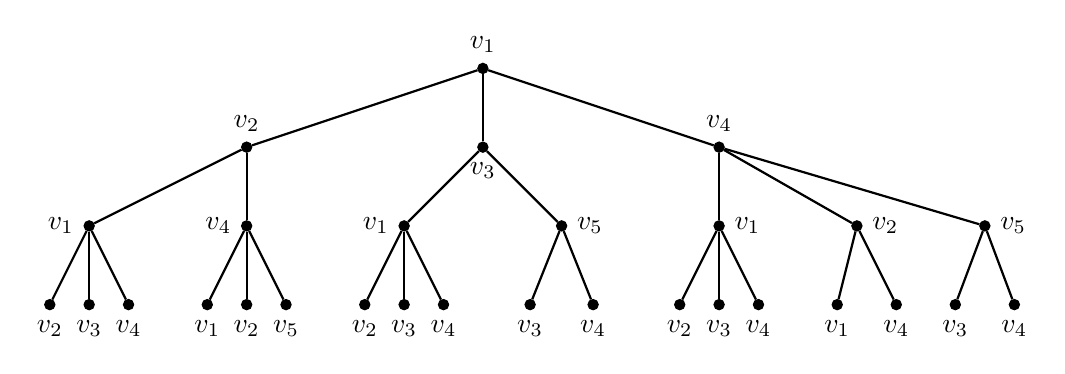
\begin{tikzpicture}

      \tikzset{enclosed/.style={draw, circle, inner sep=0pt, minimum size=.13cm, fill=black}}
%% Vertices
      	\node[enclosed, label={above: $v_1$}] (v1) at (3,6) {};
      	\node[enclosed, label={above: $v_2$}] (v2) at (0,5) {};
    		\node[enclosed, label={below: $v_3$}] (v3) at (3,5) {};
  	    \node[enclosed, label={above: $v_4$}] (v4) at (6,5) {};
     	\node[enclosed, label={left: $v_1$}] (v5) at (-2,4) {};
     	\node[enclosed, label={left: $v_4$}] (v6) at (0,4) {};
     	\node[enclosed, label={left: $v_1$}] (v7) at (2,4) {};
     	\node[enclosed, label={right: $v_5$}] (v8) at (4,4) {};
     	\node[enclosed, label={right: $v_1$}] (v9) at (6,4) {};
     	\node[enclosed, label={right: $v_2$}] (v10) at (7.75,4) {};
     	\node[enclosed, label={right: $v_5$}] (v11) at (9.375,4) {};
     	\node[enclosed, label={below: $v_2$}] (v12) at (-2.5,3) {};
      	\node[enclosed, label={below: $v_3$}] (v13) at (-2,3) {};
  	    \node[enclosed, label={below: $v_4$}] (v14) at (-1.5,3) {};
  	    \node[enclosed, label={below: $v_1$}] (v15) at (-0.5,3) {};
     	\node[enclosed, label={below: $v_2$}] (v16) at (0,3) {};
     	\node[enclosed, label={below: $v_5$}] (v17) at (0.5,3) {};
     	\node[enclosed, label={below: $v_2$}] (v18) at (1.5,3) {};
      	\node[enclosed, label={below: $v_3$}] (v19) at (2,3) {};
  	    \node[enclosed, label={below: $v_4$}] (v20) at (2.5,3) {};
  	    \node[enclosed, label={below: $v_3$}] (v21) at (3.6,3) {};
  	    \node[enclosed, label={below: $v_4$}] (v22) at (4.4,3) {};
  	    \node[enclosed, label={below: $v_2$}] (v23) at (5.5,3) {};
      	\node[enclosed, label={below: $v_3$}] (v24) at (6,3) {};
  	    \node[enclosed, label={below: $v_4$}] (v25) at (6.5,3) {};
  	    \node[enclosed, label={below: $v_1$}] (v26) at (7.5,3) {};
     	\node[enclosed, label={below: $v_4$}] (v27) at (8.25,3) {};
     	\node[enclosed, label={below: $v_3$}] (v28) at (9,3) {};
     	\node[enclosed, label={below: $v_4$}] (v29) at (9.75,3) {};
%Edges
		\path[thick] (v1) edge node[midway, sloped, above] {} (v2);
		\path[thick] (v1) edge node[midway, sloped, above] {} (v3);
		\path[thick] (v1) edge node[midway, above] {} (v4);
		\path[thick] (v2) edge node[near end, sloped, below] {} (v5);
		\path[thick] (v2) edge node[midway, below] {} (v6);
		\path[thick] (v3) edge node[near end, sloped, above] {} (v7);
		\path[thick] (v3) edge node[near end, sloped, above] {} (v8);
		\path[thick] (v4) edge node[near end, sloped, above] {} (v9);
		\path[thick] (v4) edge node[near end, sloped, above] {} (v10);
		\path[thick] (v4) edge node[near end, sloped, above] {} (v11);
		\path[thick] (v5) edge node[near end, sloped, above] {} (v12);
		\path[thick] (v5) edge node[near end, sloped, above] {} (v13);
		\path[thick] (v5) edge node[near end, sloped, above] {} (v14);
		\path[thick] (v6) edge node[near end, sloped, above] {} (v15);
		\path[thick] (v6) edge node[near end, sloped, above] {} (v16);
		\path[thick] (v6) edge node[near end, sloped, above] {} (v17);
		\path[thick] (v7) edge node[near end, sloped, above] {} (v18);
		\path[thick] (v7) edge node[near end, sloped, above] {} (v19);
		\path[thick] (v7) edge node[near end, sloped, above] {} (v20);
		\path[thick] (v8) edge node[near end, sloped, above] {} (v21);
		\path[thick] (v8) edge node[near end, sloped, above] {} (v22);
		\path[thick] (v9) edge node[near end, sloped, above] {} (v23);
		\path[thick] (v9) edge node[near end, sloped, above] {} (v24);
		\path[thick] (v9) edge node[near end, sloped, above] {} (v25);
		\path[thick] (v10) edge node[near end, sloped, above] {} (v26);
		\path[thick] (v10) edge node[near end, sloped, above] {} (v27);
		\path[thick] (v11) edge node[near end, sloped, above] {} (v28);
		\path[thick] (v11) edge node[near end, sloped, above] {} (v29);

	\end{tikzpicture}
	\caption{De mulige løsninger for veje med længde 3 fra $v_{0}$ til $v_{k}$.}
	\label{fig.vaegtetopg}
\end{figure}

Antallet af veje fra $v_{1}$ til $v_{3}$ er 5, og antallet af veje fra $v_{1}$ til $v_{4}$ er 6. Vi kan derfor opstille
\textbf{$A^{4}$}$=b_{i1} a_{1j}+b_{i2} a_{2j}=5 \cdot 1+6 \cdot 1=11$.
Her er $b_{i1}$ antallet af veje fra $v_{1}$ til $v_{3}$, og $a_{1j}$ er antallet af kanter fra $v_{3}$ til  $v_{5}$. På samme måde optræder $b_{i2}$ og $a_{2j}$ for $v_{4}$. Der er altså 11 veje med længden 4 fra $v_{1}$ til $v_{5}$.

\end{exmp}

\input{incl/main/grafer/vægtede}

\section{Delte grafer}
I visse tilfælde kan en graf deles op, for at optimere en algoritme til løsningen af problemet i en given problemstilling. \\
To måder at dele en graf op er $k$-delte grafer og delgrafer.

\begin{defn} \label{defn:k-delt} %k-partite
En graf G kaldes en $k$-delt graf $G = (V_1, V_2, \ldots, V_k; E)$, hvis følgende betingelser opfyldes: $V= V_i \cup V_j, V_i \cap V_j = Ø \forall i,j$, og $i\neq j$ 
\end{defn}

En $k$-delt graf består af $k$ disjunkte, ikke-tomme delmængder, $V_1, V_2, \ldots, V_k$, hvor for 2 vilkårlige knuder, $u$ og $v$, kun er forbundet, hvis de er i forskellige delmængder.
\begin{defn}	 \label{defn:delgraf} %subgraph
En delgraf af grafen $G= (V,E)$ er en graf $D = (W,F)$ skabt af delelementerne af kanterne og knuderne: $W \subseteq V og F \subseteq E$.
\end{defn}

Fordelen ved at dele en graf op i forskellige delgrafer er, at når man i $korteste-vej$, eller i bestemte tilfælde $længste-vej$, kan finde den optimale delstruktur hvis den optimale delgraf er fundet. Altså finder man den optimale vej igennem knuderne $(a, c, g, n)$, er den optimale vej også fundet til de mellemliggende knuder også fundet, altså fra $a$ til fx $g$.






